Dans ce chapitre, on décrit le support de notre travail: un langage impératif
nommé \langname, sur lequel s'appuieront les analyses de typage des
chapitres~\ref{cha:typbase} et~\ref{cha:qualifs}.

Le langage C~\cite{KandR} est un langage impératif, conçu pour être un
\enquote{assembleur portable}. Ses types de données et les opérations associées
sont donc naturellement de très bas niveau.

Ses types de données sont établis pour représenter les mots mémoire manipulables
par les processeurs : essentiellement des entiers et flottants de plusieurs
tailles. Les types composés correspondent à des zones de mémoire contigües,
homogènes (dans le cas des tableaux) ou hétérogènes (dans le cas des
structures).

Une des spécificités de C est qu'il expose au programmeur la notion de pointeur,
c'est-à-dire des variables qui représentent directement une adresse en mémoire.
Les pointeurs peuvent être typés (on garde une indication sur le type de l'objet
stocké à cette adresse) ou \enquote{non typés}. Dans ce dernier cas, ils ont en
fait le type \texttt{void *} qui est compatible avec n'importe quel type
pointeur.

Son système de types rudimentaire ne permet pas d'avoir beaucoup de garanties
sur la sûreté du programme. En effet, aucune vérification n'est effectuée en
dehors de celles faites par le programmeur.

Le but ici est de définir \langname, un langage plus simple mais qui permettra
de raisonner sur une certaine classe de programmes C.

Tout d'abord, on commence par présenter les notations qui accompagneront le
reste des chapitres. Cela inclut la notion de lentille, qui est utilisée pour
définir les accès profonds à la mémoire. Cela permet de résoudre le problème de
mettre à jour une sous-valeur (par exemple un champ de structure) d'une
variable, par exemple. Les lentilles permettent de définir de manière
déclarative que pour faire cette opération, il faut obtenir l'ancienne valeur de
la variable, puis calculer une nouvelle valeur en remplaçant une sous-valeur,
avant de replacer cette nouvelle valeur à sa place en mémoire. En pratique, on
définira deux lentilles: une qui relie un état mémoire à la valeur d'une
variable, et une qui relie une valeur à une de ses sous-valeurs. Avec cette
technique, on peut définir en une seule fois les opération de lecture et
d'écriture de sous-valeurs imbriquées.

Ensuite, on présente \langname en soi, c'est-à-dire sa syntaxe, ainsi qu'une
description de ses caractéristiques principales. En particulier, le modèle
mémoire est détaillé, ainsi que les valeurs manipulées par le langage.

Enfin, on décrit une sémantique opérationnelle pour ce langage. Cela permet de
définir précisément l'exécution d'un programme \langname au niveau de la
mémoire.

L'implantation de ces analyses est faite dans le chapitre~\ref{cha:implem}. En
particulier, on y verra comment traduire un sous-ensemble de C vers \newspeak,
sur lequel notre implantation est faite.

\section{Notations}

\subsection*{Inférence}

La sémantique opérationnelle consiste en la définition d'une relation de
transition $\cdot\rightarrow\cdot$ entre états de l'interprète\footnote{Dans le
chapitre~\ref{cha:typbase}, la relation de typage $\cdot ⊢ \cdot : \cdot$ sera
définie par la même technique.}.

Cette relation est définie inductivement sur la syntaxe du programme. Plutôt que
de présenter l'induction explicitement, elle est représentée par des jugements
logiques et des règles d'inférence, de la forme:

\[
\irule{Nom}{P_1 \\ … \\ P_n}{C}
\]

Les $P_i$ sont les prémisses, et $C$ la conclusion. Cette règle s'interprète de
la manière suivante: si les $P_i$ sont vraies, alors $C$ est vraie.

Certaines règles n'ont pas de prémisse, ce sont des axiomes:

\[
\iaxiom{Ax}{A}
\]

Compte-tenu de la structure des règles, la dérivation d'une preuve (l'ordre dans
lequel les règles sont appliquées) pourra donc être vue sous la forme d'un arbre
où les axiomes sont les feuilles, en haut, et la conclusion est la racine, en
bas.

\[
  \irule{r1}{
    \irule{r2}
          {
            \iaxiom{r3}{A_1}
              \\
            \iaxiom{r4}{A_2}
          }
          {B_1}
    \\
    \irule{r5}
      {
        \iaxiom{r6} {A_3}
      }{B_2}
      }{C}
\]

\subsection*{Listes}
\label{page:def-listes}

$X^*$ est l'ensemble des suites finies de $X$, indexées à partir de 1. Si $u ∈
X^*$, on note $|u|$ le nombre d'éléments de $u$ (le cardinal de son domaine de
définition). Pour $i ∈ [1 ; |u|]$, on note $u_i = u(i)$ le i-ème élément de la
suite.

On peut aussi voir les suites comme des listes: on note $[]$ la suite vide,
telle que $|[]| = 0$. On définit en outre la construction de suite de la manière
suivante: si $x ∈ X$ et $u ∈ X^*$, la liste $x::u ∈ X^*$ est la liste $v$ telle
que:

\begin{align*}
                       v_1 & = x \\
  ∀ i ∈ [1; |u|] , v_{i+1} & = u_i
\end{align*}

Cela signifie que la tête de liste ($x$ dans la liste $x :: u$) est toujours
accessible à l'indice $1$.

\subsection*{Lentilles}

Dans la définition de la sémantique de \langname, on utilise des \emph{lentilles
bidirectionnelles}. Cette notion n'est pas propre à la sémantique des
programmes. Il s'agit d'une technique permettant de relier la modification d'un
objet à la modification d'un de ses sous-composants. Cela a plusieurs
applications possibles. En programmation fonctionnelle pure (sans mutation), on
ne peut pas mettre à jour partiellement les valeurs composées comme des
enregistrements (\emph{records}). Pour simuler cette opération, on a en général
une opération qui permet de définir un nouvel enregistrement dans lequel seul un
champ a été mis à jour. C'est ce qui se passe avec le langage
Haskell~\link{haskell}: \texttt{r \{ x = 5 \}} représente une valeur
enregistrement égale à \texttt{r} sur tous les champs, sauf pour le champ
\texttt{x} où elle vaut \texttt{5}. Utiliser des lentilles revient à ajouter
dans le langage la notion de champ en tant que valeur de première classe. Elles
ont l'avantage de pouvoir se composer, c'est à dire que si on a un champ nommé
$x$ qui contient un champ nommé $y$, alors on peut modifier le champ du champ
automatiquement.

Dans ce cadre, les lentilles ont été popularisées par Van
Laarhoven~\cite{LaarhovenLenses}. Puisque cela sert à manipuler des données
arborescentes, on peut aussi appliquer cet outil aux systèmes de bases de
données ou aux documents structurés comme par exemple en
XML~\cite{PierceLenses}.

Dans notre cas, cela permettra par exemple de modifier un élément d'un tableau
qui est un champ de structure de la variable nommée $x$ dans le 3\ieme cadre de
pile.

\begin{definition}[Lentille]

Étant donnés deux ensembles $R$ et $A$, une \emph{lentille} $ℒ ∈ \setLens{R}{A}$
(ou \emph{accesseur}) est un moyen d'accéder en lecture ou en écriture à une
sous-valeur de type $A$ au sein d'une valeur de type $R$ (pour \emph{record}).
Elle est consistuée des opérations suivantes:

\begin{itemize}
\item
  une fonction de lecture $\mathrm{get}_ℒ : R → A$
\item
  une fonction de mise à jour $\mathrm{put}_ℒ : (A × R) → R$
\end{itemize}

telles que pour tous $a∈A, a'∈A, r∈R$:

\begin{align*}
\tag{\textsc{GetPut}}
\mathrm{put}_ℒ(\mathrm{get}_ℒ(r), r) &= r \\
\tag{\textsc{PutGet}}
\mathrm{get}_ℒ(\mathrm{put}_ℒ(a, r)) &= a \\
\tag{\textsc{PutPut}}
\mathrm{put}_ℒ(a', \mathrm{put}_ℒ(a, r)) &= \mathrm{put}_ℒ(a', r) \\
\end{align*}

On note $ℒ =
\mkLens{\mathrm{get}_{ℒ}}{\mathrm{put}_{ℒ}}$.

\textsc{GetPut} signifie que si on lit une valeur puis qu'on la réécrit, l'objet
n'est pas modifié; \textsc{PutGet} décrit l'opération inverse: si on écrit
une valeur dans le champ, c'est la valeur qui sera lue; enfin, \textsc{PutPut}
évoque le fait que chaque écriture est totale: quand deux écritures se suivent,
seule la seconde compte.

\end{definition}

Une illustration se trouve dans la figure~\ref{fig:lens-howto}.

\begin{figure}[h]

\tikzstyle{lenspatA}=[fill=white,pattern=crosshatch dots]
\tikzstyle{lenspatB}=[fill=blue!50]
\tikzstyle{lenspatC}=[fill=red!20]

  \begin{align*}
  \lensGet{ℒ}{\lensNodeBig{lenspatA}{lenspatB}} &= \lensInner{lenspatB} \\
  \lensPut{ℒ}{\lensInner{lenspatC}}{\lensNodeBig{lenspatA}{lenspatB}}
        &= \lensNodeBig{lenspatA}{lenspatC} \\
  \end{align*}

\caption{Fonctionnement d'une lentille}
\label{fig:lens-howto}
\end{figure}

\begin{example}[Lentilles de tête et de queue de liste]

Soit $E$ un ensemble. On considère $L(E)$, l'ensemble des listes d'éléments de
$E$.

On définit les fonctions suivantes. Notons qu'elles ne sont pas définies sur la
liste vide $[]$, qui pourra être traitée comme un cas d'erreur.

\begin{align*}
  \mathrm{get}_T     (t::q) &= t   & \mathrm{put}_T (t', t::q) &= t'::q  \\
  \mathrm{get}_Q     (t::q) &= q   & \mathrm{put}_Q (q', t::q) &= t::q'
\end{align*}

Alors
$T = \mkLens{\mathrm{get}_T}{\mathrm{put}_T} ∈ \setLens{L(E)}{E}$
et
$Q = \mkLens{\mathrm{get}_Q}{\mathrm{put}_Q} ∈ \setLens{L(E)}{L(E)}$.

On a par exemple:

\begin{align*}
\mathrm{get}_T (1::6::1::8::[]) &= 1   &   \mathrm{put}_Q (4::2::[], 3::6::1::5::[]) = 3::4::2::[]
\end{align*}

\end{example}

\begin{definition}[Lentille indexée]

Les objets de certains ensembles $R$ sont composés de plusieurs sous-objets
accessibles à travers un indice $i ∈ I$. Une lentille indexée est une fonction
$Δ$ qui associe à un indice $i$ une lentille entre $R$ et un de ses champs
$A_i$:

\[
  ∀ i ∈ I, ∃ A_i, Δ(i) ∈ \setLens{R}{A_i}
\]

On note alors:

\begin{align*}
    r {[ i ]}_Δ     & \eqdef \mathrm{get}_{Δ(i)}(r) \\
    r {[ i ← a ]}_Δ & \eqdef \mathrm{put}_{Δ(i)}(a, r) \\
\end{align*}

\end{definition}

Un exemple est illustré dans la figure~\ref{fig:lens-idx-ex}.

\begin{figure}[h]

% N&B
%\tikzstyle{lenspatA}=[fill=white,pattern=crosshatch dots]
%\tikzstyle{lenspatB}=[fill=black!50]
%\tikzstyle{lenspatC}=[fill=black!20]
\tikzstyle{lenspatA}=[fill=white,pattern=crosshatch dots]
\tikzstyle{lenspatB}=[fill=blue!50]
\tikzstyle{lenspatC}=[fill=red!20]

  \begin{align*}
    \lensGet{Δ(b)}{\lensNodeBigIdx{lenspatA}{lenspatB}{lenspatB}{lenspatB}{lenspatB}} &= \lensInnerStar{lenspatB} \\
    \lensGet{Δ(c)}{\lensNodeBigIdx{lenspatA}{lenspatB}{lenspatB}{lenspatB}{lenspatB}} &= \lensInner{lenspatB} \\
    \lensPut{Δ(b)}{\lensInnerStar{lenspatC}}{\lensNodeBigIdx{lenspatA}{lenspatB}{lenspatB}{lenspatB}{lenspatB}} &=
      \lensNodeBigIdx{lenspatA}{lenspatB}{lenspatC}{lenspatB}{lenspatB} \\
    \lensPut{Δ(c)}{\lensInner{lenspatC}}{\lensNodeBigIdx{lenspatA}{lenspatB}{lenspatB}{lenspatB}{lenspatB}} &=
      \lensNodeBigIdx{lenspatA}{lenspatB}{lenspatB}{lenspatC}{lenspatB}
  \end{align*}

\caption{Fonctionnement d'une lentille indexée}
\label{fig:lens-idx-ex}
\end{figure}

\begin{example}[Lentille \enquote{$n$\ieme élément d'un tuple}]

Soient $n ∈ ℕ$, et $n$ ensembles $E_1, …, E_n$.

Pour tout $i ∈ [1; n]$, on définit:

\begin{align*}
   g_i((x_1, …, x_n)) &= x_i \\
p_i(y, (x_1, …, x_n)) &= (x_1, …, x_{i-1}, y, x_{i+1}, …, x_n)\\
\end{align*}

Définissons $T(i) = \mkLens{g_i}{p_i}$. Alors $T(i) ∈ \setLens{(E_1×…×E_n)}{E_i}$.

Donc $T$ est une lentille indexée, et on a par exemple:

\begin{align*}
(3,1,4,1,5) {[2]}_T &= \mathrm{get}_{T(2)} ((3, 1, 4, 1, 5)) \\
                    &= 1 \\
\\
(9,2,6,5,3) {[3 ← 1]}_T &= \mathrm{put}_{T(3)} (1, (9,2,6,5,3)) \\
                        &= (9,2,1,5,3)
\end{align*}
\end{example}

La notation $3 ← 1$ peut surprendre, mais il s'interprète de la manière
suivante: en remplaçant l'élément d'indice $3$ par $1$.

\begin{definition}[Composition de lentilles]
\label{def:lens-comp}

  Soient $ℒ_1 ∈ \setLens{A}{B}$ et $ℒ_2 ∈ \setLens{B}{C}$.

  La composition de $ℒ_1$ et $ℒ_2$ est la lentille
  $ℒ ∈ \setLens{A}{C}$ définie de la manière suivante:

  \begin{align*}
    \mathrm{get}_{ℒ} (r) &=
        \mathrm{get}_{ℒ_2}
        (\mathrm{get}_{ℒ_1} r) \\
    \mathrm{put}_{ℒ} (a, r) &=
        \mathrm{put}_{ℒ_1} (\mathrm{put}_{ℒ_2}
        (a, \mathrm{get}_{ℒ_1} r), r) \\
  \end{align*}

  On notera alors $ℒ = ℒ_1 \ggg ℒ_2$ (\enquote{$ℒ_1$ flèche $ℒ_2$}).

\end{definition}

\begin{figure}[h]

\centering

%N&B
%\tikzstyle{lensInnerBefore}=[fill=black!85]
%\tikzstyle{lensInnerAfter}=[fill=black!10]
%\tikzstyle{lensMid}=[fill=black!50]
%\tikzstyle{lensExt}=[fill=white,pattern=crosshatch dots]

\tikzstyle{lensInnerBefore}=[fill=green!85]
\tikzstyle{lensInnerAfter}=[fill=orange!30]
\tikzstyle{lensMid}=[fill=blue!50]
\tikzstyle{lensExt}=[fill=white,pattern=crosshatch dots]

\shorthandoff{!}
\vspace{5mm}
\begin{tikzpicture}
[node distance=2cm
,bignode/.style={draw,shape=rectangle,minimum size=1cm,lensExt}
,smallnode/.style={draw,shape=circle,minimum size=8mm,lensMid}
,trinode/.style={draw,shape=regular polygon,regular polygon sides=3}
]

\node[bignode] (A) {};
\node[right of=A,smallnode] (B) {};
\node[right of=B,trinode,lensInnerAfter] (C) {};
\node[below of=B,smallnode] (D) {};
\node[below of=A,node distance=4cm,bignode] (E) {};

\draw[->] (A) to node[auto] {$\mathrm{get}_{ℒ_1}$} (B);
\draw[->] (B) to (D);
\draw[->] (A) to (E);
\draw (C) |- node[auto,near end,swap] {$\mathrm{put}_{ℒ_2}$} ($(B)!0.5!(D)$);
\draw (D) |- node[auto,near end,swap] {$\mathrm{put}_{ℒ_1}$} ($(A)!0.75!(E)$);

\node[smallnode] at (A) {};
\node[trinode,lensInnerBefore] at (A) {};

\node[trinode,lensInnerBefore] at (B) {};

\node[trinode,lensInnerAfter] at (D) {};

\node[smallnode] at (E) {};
\node[trinode,lensInnerAfter] at (E) {};

\node[left of=A, node distance=4cm,bignode] (GA) {};
\node[below of=GA,smallnode] (GB) {};
\node[below of=GB,trinode,lensInnerBefore] (GC) {};

\node[smallnode] at (GA) {};

\node[trinode, lensInnerBefore] at (GA) {};
\node[trinode, lensInnerBefore] at (GB) {};

\draw [->] (GA) to node[auto] {$\mathrm{get}_{ℒ_1}$} (GB);
\draw [->] (GB) to node[auto] {$\mathrm{get}_{ℒ_2}$} (GC);

\end{tikzpicture}
\vspace{5mm}
\shorthandoff{!}

\caption{Composition de lentilles}
\label{fig:compo-lens}
\end{figure}

Cette définition est illustrée dans la figure~\ref{fig:compo-lens}. Une preuve
que la composition est une lentille est donnée en annexe~\ref{proof:compo-lens}.

\section{Syntaxe}

Les figures~\ref{fig:stx-data} et~\ref{fig:stx} présentent
notre langage intermédiaire. Il contient la plupart des fonctionnalités
présentes dans les langages impératifs comme C.

\begin{figure}%{{{

  \figstxdata{}

  \caption{Syntaxe des expressions}
\label{fig:stx-data}
\end{figure}%}}}

Parmi les expressions, les constantes comportent les entiers et flottants, ainsi
que le pointeur \eNull qui correspond à une valeur par défaut pour les
pointeurs, et la valeur unité \eUnit qui pourra être retournée par les fonctions
travaillant par effets de bord uniquement.

Les accès mémoire en lecture et écriture se font au travers de valeurs gauches
(\emph{left values} ou \emph{lvalues}): comme en C, elles tiennent leur nom du
fait que ce sont ces constructions qui sont à gauche du signe d'affectation. En plus
des variables, on obtient une valeur gauche en accédant par nom à un champ ou par
indice à un élément d'une valeur gauche, ou encore en appliquant l'opérateur
\texttt{*} de déréférencement à une expression. Pour assister le typage, l'accès
à un champ doit être décoré du type complet $S$, mais cette annotation est
ignorée lors de l'évaluation. Les valeurs gauches correspondent aussi à l'unité
d'adressage: c'est-à-dire que les pointeurs sont construits en prenant l'adresse
d'une valeur gauche avec l'opérateur \texttt{\&}.

Les fonctions sont des expressions comme les autres, contrairement à C où elles
sont forcément déclarées globalement. Cela veut dire qu'on peut affecter une
fonction $f$ à une variable $x$ et l'appeller avec $x(a_1, a_2)$. Il est aussi
possible de déclarer une fonction au sein d'une fonction. Cependant cela ne
respecte pas l'imbrication lexicale: dans la fonction interne il n'est pas
possible de faire référence à des variables locales de la fonction externe,
seulement à des variables globales. En mémoire les fonctions sont donc
uniquement représentées par leur code: il n'y a pas de fermetures.

Enfin, on trouve aussi des expressions permettant de construire des valeurs
composées: les structures et les tableaux.

\begin{figure}%{{{

  \figstxinstr{}

  \caption{Syntaxe des instructions}
\label{fig:stx}
\end{figure}%}}}

Les instructions sont typiques de la programmation impérative. \langname
comporte bien sûr l'instruction vide qui ne fait rien et la séquence qui chaîne
deux instructions.

Une expression peut être évaluée dans un contexte d'instruction, pour ses effets
de bord. Remarquons que l'affectation n'est pas présente ici: c'est en effet une
expression, qui renvoie la valeur qui a été affectée. Cela permet d'écrire $x ←
(y ← z)$, comme dans un programme C où on écrirait \texttt{x = y = z}.

Il est également possible de déclarer une variable locale avec
$\iDecl{x}{v}{i}$. $x$ est alors une nouvelle variable visible dans $i$ avec
pour valeur initiale $v$.

L'alternative et la conditionnelle sont classiques; en revanche, on ne fournit
qu'un seul type de boucle et pas de saut (instruction \texttt{goto}).

Les opérateurs sont donnés dans la figure~\ref{fig:stx-ops}. Ils correspondent à
ceux du langage C. La différence principale est que les opérations sur les
entiers, flottants et pointeurs sont annotés avec le type de données sur lequel
ils travaillent. Par exemple \enquote{$+$} désigne l'addition sur les entiers et
\enquote{$+.$} l'addition sur les flottants. Les opérations de test d'égalité,
en revanche, sont possibles pour les types numériques, les pointeurs, ainsi que
les types composés de types comparables.

\begin{figure}[h]%{{{

  \figstxops{}

  \caption{Syntaxe des opérateurs}
\label{fig:stx-ops}
\end{figure}%}}}

\section{Mémoire et valeurs}

L'interprète que nous nous apprêtons à définir manipule des valeurs qui sont
associées aux variables du programme.

La mémoire est constituée de variables (toutes mutables), qui contiennent des
valeurs. Ces variables sont organisées, d'une part en un ensemble de variables
globales, et d'autre part en une pile de contextes d'appel (qu'on appellera donc
aussi cadres de pile, ou \emph{stack frames} en anglais). Cette structure
empilée permet de représenter les différents contextes à chaque appel de
fonction: par exemple, si une fonction s'appelle récursivement, plusieurs
instances de ses variables locales sont présentes dans le programme. Le modèle
mémoire présenté ici de permet pas l'allocation dynamique sur un tas. Cette
limitation sera détaillée dans le chapitre~\ref{cha:conclusion}.

La structure de pile des locales permet de les organiser en niveaux
indépendants: à \linebreak chaque appel de fonction, un nouveau cadre de pile
est créé, comprenant ses paramètres et ses variables locales. Au contraire, pour
les globales il n'y a pas de système d'empilement, puisque ces variables sont
accessibles depuis tout point du programme.

Pour identifier de manière non ambigüe une variable, on note simplement $x$ la
variable globale nommée $x$, et $(n, x)$ la variable locale nommée $x$ dans le
$n$\ieme cadre de pile\footnote{Les paramètres de fonction sont traités comme
des variables locales et se retrouvent dans le cadre correspondant.}.

Les affectations peuvent avoir la forme $x ← e$ où $x$ est une variable et $e$
est une expression, mais pas seulement. En effet, à gauche de $←$ on trouve en
général non pas une variable mais une valeur gauche (par définition). Pour
représenter quelle partie de la mémoire doit être accédée par cette valeur
gauche, on introduit la notion de chemin $φ$. Un chemin est une valeur gauche
évaluée: les cas sont similaires, sauf que tous les indices sont évalués. Par
exemple, $φ = (5, x).p$ représente le champ \enquote{$p$} de la variable $x$
dans le 5\ieme cadre de pile. C'est à ce moment qu'on évalue les
déréférencements qui peuvent apparaître dans une valeur gauche.

Les valeurs, quant à elles, peuvent avoir les formes suivantes (résumées sur la
figure~\ref{fig:interp-val}):

\begin{itemize}
\item

$\widehat{c}$: une constante. La notation circonflexe permet de distinguer
les constructions syntaxique des constructions sémantiques. Par exemple, à la
syntaxe $3$ correspond la valeur $\widehat{3}$.

\label{page:entiers-bits}
Les valeurs entières sont les entiers signés sur 32 bits, c'est-à-dire entre
$-2^{31}$ à $2^{31}-1$. Mais ce choix est arbitraire: on
aurait pu choisir des nombres à 64 bits, par exemple.
Les flottants sont les flottants IEEE 754 de 32 bits~\cite{ieee754}.

Il n'y a pas de distinction entre procédures et fonctions; toutes les fonctions
doivent renvoyer une valeur. Celles qui ne retournent pas de valeur
\enquote{intéressante} renvoient alors une valeur d'un type à un seul élément
noté \eUnit\footnote{Cette notation évoque un $n$-uplet à 0 composante.}, et
donc le type sera noté \tUnit.

\item

$\widehat{\&}~φ$: une référence mémoire. Ce chemin correspond à un pointeur sur
une valeur gauche. Par exemple, l'expression $\&x$ s'évalue en $\widehat{\&}~φ =
\widehat{\&}~(5, x)$ si $x$ désigne lexicalement une variable dans le 5\ieme
cadre de pile.

\item

$\widehat{ \eArray{v_1 ;…; v_n} }$: un tableau. C'est une valeur composée qui
contient un certain nombre (connu à la compilation) de valeurs d'un même type,
par exemple 100 entiers. On accède à ces valeurs par un indice entier. C'est une
erreur ($\serr{array}$) d'accéder à un tableau en dehors de ses bornes,
c'est-à-dire en dehors de $[0;n-1]$ pour un tableau à $n$ éléments.
Pareillement, $\widehat{\eArray{\cdot}}$ permet de désigner les valeurs tableau.
Par exemple, si $x$ vaut $2$ et $y$ vaut $3$, l'expression $\eArray{ x, y }$
s'évaluera en la valeur $\widehat{\eArray{ 2, 3 }}$

\item

$\widehat{ \eStruct{ l_1 : v_1 ; … ; l_n : v_n } }$: une structure. C'est une
valeur composée mais hétérogène. Les différents éléments (appelés \emph{champs})
sont désignés par leurs noms $l$ (pour \emph{label}). Dans le programme, le nom de
champ $l$ est décoré de la définition complète de la structure $S$. Celle-ci
n'est pas utilisée dans l'évaluation et sera décrite au
chapitre~\ref{cha:typbase}. Comme précédemment, on note
$\widehat{\eStruct{\cdot}}$ pour dénoter les valeurs.

\item

$\widehat{f}$: une fonction. On garde en mémoire l'intégralité de la définition
de la fonction (liste de paramètres, de variables locales et corps). Même si les
fonctions locales sont possibles, il n'est pas possible d'accéder aux variables
de la portée entourante depuis la fonction intérieure (il n'y a pas de
fermetures). Contrairement à C, les fonctions ne sont pas des cas spéciaux. Par
exemple, les fonctions globales sont simplement des variables globales de type
fonctionnel, et les \enquote{pointeurs sur fonction} de C sont remplacés par des
variables de type fonction.

\item $Ω$: une erreur. Par exemple le résultat de $5 / 0$ est $\serr{div}$.

\end{itemize}

\begin{figure}%{{{

  \begin{align*}
  \gramdef{Valeurs}{v}
      { \widehat{c}     }{Constante}
      { \widehat{\&}~φ  }{Référence mémoire}
      { \widehat{
         \eStruct{ l_1 : v_1 ;
       … ; l_n : v_n }
       }                }{Structure}
      { \widehat{
        \eArray{v_1 ;…; v_n}
        }               }{Tableau}
      { \widehat{f}     }{Fonction}
      { Ω               }{Erreur}
      {END}
  \\
  \\
  \gramdef{Chemins}{φ}
     { a    }{Adresse}
     { φ\widehat{.}l  }{Accès à un champ}
     { φ\widehat{[n]} }{Accès à un élément}
     {END}
  \\
  \\
  \gramdef{Adresses}{a}
     { (n, x) }{Variable locale}
     { (x)    }{Variable globale}
     {END}
  \\
  \\
  \gramdef{Erreur}{Ω}
    { \serr{array} }{Débordement de tableau}
    { \serr{ptr}   }{Erreur de pointeur}
    { \serr{div}   }{Division par zéro}
    { \serr{field} }{Erreur de champ}
    { \serr{var}   }{Variable inconnue}
    { \serr{typ}   }{Données incompatibles}
    {END}
  \end{align*}

  \caption{Valeurs}
\label{fig:interp-val}
\end{figure}%}}}

Les erreurs peuvent être classifiées en deux grand groupes: d'une part,
$\serr{field}$, $\serr{var}$ et $\serr{typ}$ sont des erreurs de typage
dynamique, qui arrivent lorsqu'on accède dynamiquement à des données qui
n'existent pas ou qu'on manipule des types de données incompatibles. D'autre
part, $\serr{div}$, $\serr{array}$ et $\serr{ptr}$ correspondent à des valeurs
mal utilisées. Le but du système de types du chapitre~\ref{cha:typbase} sera
d'éliminer complètement les erreurs du premier groupe.

\section{Interprète}

La figure~\ref{fig:interp-stack} résume comment ces valeurs sont organisées. Une
pile est une liste de cadres de piles, et un cadre de pile est une liste de
couples (nom, valeur). Un état mémoire $m$ est un couple $(s, g)$ où $s$ est une
pile et $g$ un cadre de pile (qui représente les variables globales). On note
$|m| = |s|$ la hauteur de la pile (en nombre de cadres).

\begin{figure}%{{{

  \begin{align*}
  \gramdef{Pile}{s}
    { [] }{Pile vide}
    { \{ x_1 ↦v_1; … ; x_n ↦v_n\} :: s }{Ajout d'un cadre}
    {END}
  \\
  \\
  \gramdef{État mémoire}{m}
    { (s, \{ x_1 ↦v_1; … ; x_n ↦v_n\})}{Pile, globales}
    {END}
  \\
  \\
  \gramdef[4cm]{État d'interprète}{Ξ}
    { \msi{m}{e} }{Expression, mémoire}
    { \msi{m}{i} }{Instruction, mémoire}
    { Ω          }{Erreur}
    {END}
  \end{align*}

  \caption{Composantes d'un état mémoire}
\label{fig:interp-stack}
\end{figure}%}}}


Enfin, l'interprétation est définie comme une relation $\cdot → \cdot$ entre
états $Ξ$; ces états sont d'une des formes suivantes:

\begin{itemize}
\item
  un couple $\msi{m}{e}$ où $e$ est une expression et $m$ un état
  mémoire. $m$ est l'état mémoire sous lequel l'évaluation sera
  réalisée. Par exemple $\mm{([], [x↦3])}{3}{([], [x↦3])}{\widehat{3}}$
  L'évaluation des expressions est détaillée dans la
  section~\ref{sec:eval-exp}.
\item
  un couple $\msi{m}{i}$ où $i$ est une instruction et $m$ un état
  mémoire. La réduction des instructions est traitée dans la
  section~\ref{sec:eval-instr}.
  Par exemple, $ \msi{m}{(x ← 3 ; y ← x)} → \msi{m [x ↦ \widehat{3}]}{y ← x}
                           → \msi{m [x ↦ \widehat{3}][y ↦
    \widehat{3}]}{\iPass}$.

  Dans le cas général, utiliser des instructions pour représenter l'état des
  calculs ne suffit pas; il faut utiliser une continuation.
  C'est ce qui est fait par exemple dans la sémantique de
  CMinor~\cite{cminorSL}.
  Ici, le flot de contrôle est plus simple et on peut se contenter de retenir
  une simple instruction, ce qui simplifie la présentation.

\item
  un couple $\msi{m}{lv}$ où $lv$ est une valeur gauche et $m$ un état mémoire.
  L'évaluation des valeurs gauches est décrite en section~\ref{sec:eval-lv}.
\item
  une erreur $Ω$. La propagation des erreurs est détaillée dans la
  section~\ref{sec:eval-errors}.
\end{itemize}

L'évaluation des expressions, valeurs gauches et instructions se fait à petits
pas. C'est-à-dire qu'on simplifie d'étape en étape leur forme, jusqu'à arriver à
un cas de base:

\begin{itemize}
\item pour les expressions, une valeur $v$;
\item pour les instructions, l'instruction $\iPass$ ou $\iReturn{v}$ où $v$ est
    une valeur;
\item pour les valeurs gauches un chemin $φ$.
\end{itemize}

On considère en fait la clôture transitive de cette relation. Cela revient à
ajouter une règle :

\begin{mathpar}
    \irule{Trans}
        { Ξ_1 → Ξ_2
       \\ Ξ_2 → Ξ_3
        }
        { Ξ_1 → Ξ_3}
\end{mathpar}

\section{Opérations sur les valeurs}
\label{sec:sem-ops}

Un certain nombre d'opérations est possible sur les valeurs
(figure~\ref{fig:stx-ops}):

\begin{itemize}
\item
  les opérations arithmétiques $+$, $-$, $×$, $/$ et $\%$ sur les entiers.
  L'opérateur $\%$ correspond au modulo (reste de la division euclidienne).
  En cas de division par zéro, l'erreur $\serr{div}$ est levée.
\item
  les versions \enquote{pointées}
  $\floatop{+}$,
  $\floatop{-}$,
  $\floatop{×}$
  et
  $\floatop{/}$
  sur les flottants.
\item
  les opérations d'arithmétique de pointeur $+_p$ et $-_p$ qui à un chemin
  mémoire et un entier associent un chemin mémoire.
\item
  les opérations d'égalité $=$ et $≠$. L'égalité entre entiers ou entre
  flottants est immédiate. Deux valeurs composées (tableaux ou structures) sont
  égales si elles ont la même forme (même taille pour les tableaux, ou même
  champs pour les structures) et que toutes leurs sous-valeurs sont égales deux
  à deux. Deux références mémoire sont égales \linebreak lorsque les chemins
  qu'elles décrivent sont syntaxiquement égaux.
\item
  les opérations de comparaison $≤,≥,<,>$ sont définies avec leur sémantique
  habituelle sur les entiers et les flottants. Sur les références mémoires,
  elles sont définies dans le cas où les deux opérandes sont de la forme
  $φ[\cdot]$ par: $φ[n]~\opbin~φ[m] \eqdef n~\opbin~m$. Dans les autres cas,
  l'erreur $\serr{ptr}$ est renvoyée. Notamment, il n'est pas possible de
  comparer deux fonctions, deux tableaux ou deux structures.
\item
  les opérateurs bit à bit sont définis sur les entiers. $\&$, $|$ et $\opxor$
  représentent respectivement la conjonction, la disjonction et la disjonction
  exclusive (XOR).
\item
  des versions logiques de la conjonction ($\&\&$) et de la disjonction ($||$)
  sont également présentes. Leur sémantique est donnée par le tableau suivant:

  \begin{center}
    \begin{tabular}{rr@{\hskip 1cm}cc}
      \toprule
       $n$ &  $m$ & $n~\&\&~m$ & $n~||~m$ \\
      \midrule
       $0$ &  $0$ & $0$        & $0$      \\
       $0$ & $≠0$ & $0$        & $1$      \\
      $≠0$ &  $0$ & $0$        & $1$      \\
      $≠0$ & $≠0$ & $1$        & $1$      \\
      \bottomrule
    \end{tabular}
  \end{center}

\item
  des opérateurs de décalage à gauche ($\ll$) et à droite ($\gg$) sont présents.
  Eux aussi ne s'appliquent qu'aux entiers.

\item
  les opérateurs arithmétiques unaires $+$, $-$, $\floatop{+}$ et $\floatop{-}$
  sont équivalents par définition à l'opération binaire correspondante.
  Par exemple $\widehat{-}4 \eqdef 0\widehat{-}4$.

\item
  $\sim$ inverse tous les bits de son opérande.
  $!$ est une version logique, % chktex 40
  c'est-à-dire que $!0 = 1$ et si $n ≠ 0$, $!n = 0$.
\end{itemize}

Si ces opérateurs sémantiques reçoivent des données incompatibles (par exemple
si on tente d'ajouter une fonction et un entier), l'erreur spéciale $\serr{typ}$
est renvoyée.

\section{Opérations sur les états mémoire}
\label{sec:memops}

\begin{definition}[Recherche de variable]

  La recherche de variable permet d'associer à une variable $x$ une adresse $a$.

  Chaque fonction peut accéder aux variables locales de la fonction en cours,
  ainsi qu'aux variables globales.

  Remarque: le cadre de variables locales le plus récent a toujours l'indice $1$.

\[
  \cLookup{(s, g)}{x} =
        \begin{cases}
            (|s|, x) & \mbox{ si } |s| > 0
                       \mbox{ et } (x ↦ v) ∈ s_1 \\
            x        & \mbox{ si } (x ↦ v) ∈ g \\
            \serr{var} & \mbox{ sinon }
        \end{cases}
\]

\end{definition}

En entrant dans une fonction, on rajoutera un cadre de pile qui contient les
paramètres de la fonction ainsi que ses variables locales. En retournant à
l'appelant, il faudra supprimer ce cadre de pile.

\begin{definition}[Manipulations de pile]

  On définit l'empilement d'un cadre de pile $c = ((x_1↦ v_1), …, (x_n↦ v_n))$
  sur un état mémoire $m = (s, g)$ (figure~\ref{fig:stackops-push}):

  \[
      \cPush{(s, g)}{c} = (c::s, g)
  \]

  On définit aussi l'extension du dernier cadre de pile, qui sert aux
  déclarations de variables locales (figure~\ref{fig:stackops-extend}):

  \[
    \cExtend{(c::s, g)}{x}{v} = (((x↦v :: c) :: s), g)
  \]

  L'opération inverse de $\phxxx\cExtend$ sera simplement notée \enquote{$-$} :
  $m - x$, par exemple.

  De même on définit le dépilement (figure~\ref{fig:stackops-pop}):

  \[
      \cPop{(c::s, g)} = (s, g)
  \]

\end{definition}

\begin{definition}[Hauteur d'une valeur]
\label{def:hauteur-val}
Une valeur peut contenir une référence vers une variable de la pile.
La hauteur d'une valeur est l'indice du plus haut cadre qu'elle référence, ou
$-1$ sinon.

\begin{center}
\begin{minipage}{0.4\textwidth}
\begin{align*}
    \cH{\widehat{c}} &= -1 \\
    \cH{\widehat{f}} &= -1 \\
    \cH{\widehat{\&}~φ} &= \cHphi{φ} \\
    \cH{\widehat{\eStruct{l_1:v_1;…;l_n:v_n}}} &= \max_{i∈[1;n]} \cH{v_i} \\
    \cH{\widehat{\eArray{v_1,…,v_n}}} &= \max_{i∈[1;n]} \cH{v_i}
\end{align*}
\end{minipage}
\hspace{1.2em}
\mbox{où:}
\hspace{0.8em}
\begin{minipage}{0.3\textwidth}
\begin{align*}
    \cHphi{(x)} &= -1 \\
    \cHphi{(n,x)} &= n \\
    \cHphi{φ\widehat{.}l} &= \cHphi{φ} \\
    \cHphi{φ\widehat{[n]}} &= \cHphi{φ}
\end{align*}
\end{minipage}
\end{center}

\end{definition}


Les opérations $\mathrm{Extend}$ et $\mathrm{Pop}$ ne sont définies que pour une
pile non vide. Néanmoins cela ne pose pas de problème, puisque, lors de
l'exécution, la pile n'est vide que lors de l'évaluation d'expressions dans les
phrases de programme. À cet endroit, seules des expressions peuvent apparaître,
et leur évaluation ne manipule jamais la pile avec ces opérations.

\begin{figure}%{{{

  \centering

  \subbottom[Empilement]{
\label{fig:stackops-push}
  \begin{tikzpicture}
    [ stack/.style={draw,shape=rectangle,minimum height=5mm,minimum width=2cm}
    , every node/.style={font=\footnotesize}
    , faded/.style={fill=black!20}
    ]
    \path (8,0)   node [stack, faded] {}
    -- ++ (0,0.5) node [stack, faded] {}
    -- ++ (0,0.5) node [stack, faded] {}
    ;
    \path (12,0)  node [stack, faded] {}
    -- ++ (0,0.5) node [stack, faded] {}
    -- ++ (0,0.5) node [stack, faded] {}
    -- ++ (0,0.5) node [stack] {$x↦0$}
    ;
    \draw [->] (9.2, 1) -- node[auto] {$\cPush{\cdot}{(x ↦ 0)}$} ++(1.6, 0);
  \end{tikzpicture}
  }

  \subbottom[Extension de cadre]{
\label{fig:stackops-extend}
  \begin{tikzpicture}
    [ stack/.style={draw,shape=rectangle,minimum height=5mm,minimum width=2cm}
    , every node/.style={font=\footnotesize}
    , faded/.style={fill=black!20}
    ]
    \path (4,-3)  node [stack, faded] {}
    -- ++ (0,0.5) node [stack, faded] {}
    -- ++ (0,0.5) node [stack, faded] {}
    -- ++ (0,0.5) node [stack] {$x↦0$}
    ;
    \path (8,-3)  node [stack, faded] {}
    -- ++ (0,0.5) node [stack, faded] {}
    -- ++ (0,0.5) node [stack, faded] {}
    -- ++ (0,0.5) node [stack] {$x↦0, y↦3$}
    ;
    \draw [->] (5.2, -2) -- node[auto] {$\cExtend{\cdot}{y}{3}$} ++(1.6, 0);
  \end{tikzpicture}
  }

  \subbottom[Dépilement]{
\label{fig:stackops-pop}
  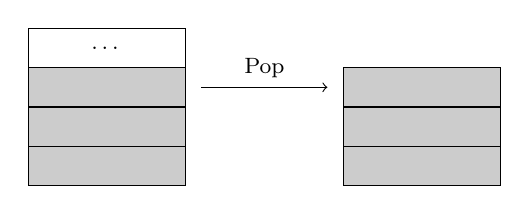
\begin{tikzpicture}
    [ stack/.style={draw,shape=rectangle,minimum height=5mm,minimum width=2cm}
    , every node/.style={font=\footnotesize}
    , faded/.style={fill=black!20}
    ]
    \path (0,0)   node [stack, faded] {}
    -- ++ (0,0.5) node [stack, faded] {}
    -- ++ (0,0.5) node [stack, faded] {}
    -- ++ (0,0.5) node [stack] {$…$}
    ;
    \path (4,0)   node [stack, faded] {}
    -- ++ (0,0.5) node [stack, faded] {}
    -- ++ (0,0.5) node [stack, faded] {}
    ;
    \draw [->] (1.2, 1) -- node[auto] {Pop} ++(1.6, 0);
  \end{tikzpicture}
  }

  \caption{Opérations de pile}
\label{fig:stackops}
\end{figure}%}}}

On définit aussi une opération de nettoyage de pile, qui sera utile pour les
retours de fonction.

En effet, si une référence au dernier cadre est toujours présente après
le retour d'une fonction, cela peut casser le typage.

Par exemple, dans la figure~\ref{fig:prog-cleanup}, l'exécution de $h()$ donne à
$p$ la valeur $(1, x)$. Puis en arrivant dans $g$, le déréférencement de $p$ va
modifier $x$ qui va avoir la valeur $1$. $x$, variable flottante, contient donc
un entier.
Dans la ligne marquée \texttt{(*)}, on réalise donc l'addition
d'un entier (contenu dans $x$ malgré son type) et d'un flottant. Cette opération
est bien typée mais provoquera une erreur $\serr{typ}$ à l'exécution.

Pour empêcher cela, on instrumente donc le retour de la fonction
\texttt{f} pour que \texttt{p} soit remplacé par $\eNull$. Alors dans
\texttt{h}, le déréférencement provoquera une erreur et empêchera la violation
du typage.

\begin{SaveVerbatim}[]{LeBonProgramme}
f = Fun () {
    Decl x = 0 in
    return (&x);
}

g = Fun (p) {
    Decl x = 0.0 in
    *p = 1;
    x <- x + 2.0; // (*)
}

h = Fun () {
    Decl p = f() in
    g(p);
}
\end{SaveVerbatim}

\begin{figure}
\hspace{1cm}\BUseVerbatim{LeBonProgramme}
\caption{Cassage du typage par un pointeur fou}
\label{fig:prog-cleanup}
\end{figure}

Pour définir l'opération de nettoyage, on commence par définir une opération
nettoyant une valeur selon un prédicat sur les chemins:

\begin{align*}
\cVP{p}{\widehat{c}} &= \widehat{c} \\
\cVP{p}{\widehat{f}} &= \widehat{f} \\
\cVP{p}{\wphi{φ}} &= \begin{cases}
                       \eNull   & \mbox{ si }    p(φ) \\
                       \wphi{φ} & \mbox{ sinon}
                     \end{cases} \\
\cVP{p}{\widehat{\eStruct{l_1:v_1, …, l_n:v_n}}} &=
    \widehat{\eStruct{l_1:\cVP{p}{v_1}, …, l_n:\cVP{p}{v_n}}} \\
\cVP{p}{\widehat{\eArray{v_1, …, v_n}}} &=
    \widehat{\eStruct{\cVP{p}{v_1}, …, \cVP{p}{v_n}}}
\end{align*}

On l'étend ensuite aux cadres de pile, puis aux états mémoire:

\begin{align*}
\cLP{p}{(x_1 ↦ v_1, …, x_n ↦ v_n)} &= (x_1 ↦ \cVP{p}{v_1}, …, x_n ↦ \cVP{p}{v_n}) \\
\\
                \cP{p}{(s, g)} &= (s', g') \\
                 \mbox{où } s' &= (\cLP{p}{s_1}, …, \cLP{p}{s_{|s|}}) \\
                            g' &=  \cLP{p}{g}
\end{align*}

À l'aide de ces fonctions, on définit quatre opérations, permettant de nettoyer
des états mémoire ou des valeurs en enlevant tout un niveau de pile ou seulement
une variable:

\begin{mathpar}
\cCleanup{m} =  \cP{λφ: \cHphi{φ} > |m|}{m}

\cCleanVar{m}{a}  = \cP{λφ: φ = a}{m}

\cV{p}{v}    = \cVP{λφ: \cHphi{φ} > |m|}{v}

\cVV{v}{a}        = \cVP{λφ: φ = a}{v}
\end{mathpar}

Ces 4 fonctions seront utilisées dans plusieurs règles dans la suite de ce
chapitre.

\paragraph{Remarques}

Ces opérations ne sont pas toujours bien définies. Par exemple, $\phxxx\cExtend$
ne peut pas s'appliquer à une pile vide, et $m - x$ n'est défini que si une
variable $x$ existe au sommet de la pile de $m$. Ce caractère partiel ne pose
pas de problème de par la structure des règles qui vont utiliser ces
constructions. Par exemple, à chaque empilement correspond exactement un
dépilement. De plus, les phrases d'un programme ne peuvent pas faire intervenir
de déclaration de variable (une instruction est forcément dans une fonction),
donc $\phxxx\cExtend$ réussit toujours.

Un autre problème se pose si deux variables ont le même nom dans un cadre. Elles
ne peuvent pas être distinguées. On interdit donc ce cas en demandant aux
programmes d'être bien formés: au sein d'une fonction, les paramètres ainsi que
l'ensemble des locales déclarées doivent être de noms différents. En pratique,
une phase préalable d'$α$-conversion peut renommer les variables problématiques.

\section{Accesseurs}
\label{sec:mem-access}

Le but de cette section est de définir rigoureusement les accès à la mémoire. À
partir d'un état mémoire $m$ et d'une valeur gauche $φ$, on veut pouvoir obtenir:

\begin{itemize}
    \item la valeur accessible au chemin $φ$: $m[φ]_Φ$
    \item l'état mémoire obtenu en remplaçant celle-ci par une nouvelle valeur $v'$ :
            $m[φ ← v']_Φ$
\end{itemize}

Pour définir cette lentille indexée $Φ$, on commence par définir des lentilles
élémentaires, et on les compose pour pouvoir définir des lentilles entre
valeurs.

On commence par définir deux lentilles $I$ et $L$ pour accéder aux structures de
listes. $I$ accède par indice et $L$ par clef (dans une liste d'association,
donc).

Cela permet ensuite de définir $A$, qui extrait une valeur à partir d'un nom de
variable et d'une éventuelle hauteur de pile. Pour cela, on compose les
lentilles $I$ et $L$.

Les autres travaillent sur des valeurs composées, c'est-à-dire sur les
structures et tableaux. La lentille $F$ extrait une sous-valeur
correspondant au champ d'une structure. Le fonctionnement est similaire à la
lentille $L$ puisqu'on accède par nom à une sous-structure.
La lentille $T$, quant à elle, permet d'accéder au $n$\ieme élement d'un
tableau. De ce point de vue, elle est similaire à $I$ mais en travaillant sur
les valeurs.

Enfin, on définit $Φ$ pour accéder à n'importe quelle sous-valeur d'une variable
dans la mémoire. Cela utilise $A$, $F$ et $T$ précédemment définis.

La figure~\ref{fig:dep-lens} résume ces dépendances. Les lignes pleines
indiquent quelles sont les définitions utilisées, et les pointillés relient les
lentilles similaires. À droite, on donne un exemple des lentilles de base. La
valeur entourée correspond au \enquote{curseur} de la lentille, c'est-à-dire la
valeur qui peut être renvoyée ou mise à jour.

\begin{figure}[h]
\centering
\vspace{5mm}
\begin{minipage}[b]{0.4\textwidth}
\begin{tikzpicture}
\node[draw] (I) {I};
\node[draw, below of=I] (L) {L};
\node[draw, below of=L] (F) {F};
\node[draw, below of=F] (T) {T};
\node[draw, right of=L, node distance=2cm, yshift=5mm] (A) {A};
\node[draw, right of=F, node distance=4cm, yshift=-5mm] (P) {$Φ$};

\draw[->] (I) -- (A.north west);
\draw[->] (L) -- (A.south west);
\draw[->] (A) -- (P.north west);
\draw[->] (F) -- (P.west);
\draw[->] (T) -- (P.south west);

\draw[dotted] (L) -- ++(-5mm,  0) |- (F);
\draw[dotted] (I) -- ++(-10mm, 0) |- (T);
\end{tikzpicture}
\end{minipage}
\begin{minipage}[b]{0.5\textwidth}
\begin{align*}
I(3)     &: (3, 14, \circled{15}, 92, 65) \\
L(toto)  &: ((toto, \circled{3}), (tata, 6), (titi, 2)) \\
F(y)     &: \{ x: 0; y: \circled{-3} \} \\
T(0)     &: \eArray{\circled{1}, 2, 3, 5} \\
\end{align*}
\end{minipage}
\vspace{5mm}

\caption{Dépendances entre les lentilles}
\label{fig:dep-lens}

\end{figure}

\paragraph{Remarque}

Dans toute la suite, on emploiera la notation $m[φ]_Φ$. Il est important de
remarquer que $m$ désigne un état particulier et $φ$ un chemin particulier, mais
que $Φ$ est la lentille indexée globale définie page~\pageref{subsec:acces-phi}.

\subsection*{Accès à une liste par indice : $I$}

On définit une lentille indexée $I : ℕ → \setLens{\textrm{List}(α)}{α}$
permettant d'accéder aux éléments d'une liste par leur indice. On rappelle que
les listes sont des suites finies, définies page~\pageref{page:def-listes}. En
outre, I n'est définie que pour $n ∈ [1 ;|l|]$.

\begin{align*}
    l{[n]}_I     &= l_n \mbox{ si } n ∈ [1; |l|] \\
    l{[n ← x]}_I &= l' \\
           \mbox{ où } & l'_n = x \\
                       & ∀ i ≠ n, l'_i = l_i
\end{align*}

\subsection*{Accès à une liste d'associations : $L$}

  Une liste d'association est une liste de paires (clef, valeur) avec
  l'invariant supplémentaire que les clefs sont uniques. Il est donc possible de
  trouver au plus une valeur associée à une clef donnée. L'écriture est
  également possible, en remplaçant un couple par un couple avec une valeur
  différente.

\begin{align*}
l{[x]}_L  &=
    \begin{cases}
        v          & \mbox{ si } ∃! n ∈ [1;|l|]. ∃v. l_n = (x ↦ v) \\
        \serr{var} & \mbox{ sinon }
    \end{cases} \\
l{[x ← v]}_L  &=
    \begin{cases}
        l{[n ← (x ↦ v')]}_I & \mbox{ si } ∃! n ∈ [1;|l|]. ∃v. l_n = (x ↦ v) \\
        \serr{var} & \mbox{ sinon }
    \end{cases} \\
\end{align*}

\subsection*{Accès par adresse : $A$}

Les états mémoire sont constitués des listes d'association (nom, valeur).

L'accesseur par adresse ${[\cdot]}_A$ permet de généraliser l'accès à ces
valeurs en utilisant comme clef non pas un nom mais une adresse.

Selon cette adresse, on accède soit à la liste des globales, soit à une
des listes de la pile des locales.

On pose $m = (s, g)$.

Les accès aux globales se font de la manière suivante. Si la variable n'existe
pas, notons que $L$ retourne $\serr{var}$.

\[
A((x)) = \mathrm{Snd} \ggg L(x)
\]

$\mathrm{Snd}$ désigne la lentille entre un couple et sa deuxième composante.
Ainsi, par exemple $m{[(x) ← v]}_A = (s, g[x←v]_L)$.

%\begin{align*}
%m {[x]}_A     &= g{[x]}_L \\
%m {[x ← v]}_A &= (s, g{[x←v]}_L) \\
%\end{align*}

Les accès aux locales reviennent à accéder à la bonne variable du bon cadre de
pile. Cela revient naturellement à composer les lentilles $L$ et $I$. On définit
donc une lentille $ℒ_{n,x} = I(|s|-n+1) \ggg L(x)$ qui accède à la variable $x$
du $n$\ieme cadre de pile.

\begin{align*}
m {[(n, x)]}_A     & = \begin{cases}
                           \lensGet{ℒ_{n,x}}{s} & \mbox{ si $n ∈ [1 ; |s|]$} \\
                           \serr{var}          & \mbox{ sinon}
                       \end{cases} \\
m {[(n, x) ← v]}_A & = \begin{cases}
                            (\lensPut{ℒ_{n,x}}{v}{s}, g) & \mbox{ si $n ∈ [1;|s|]$} \\
                            \serr{var}          & \mbox{ sinon}
                       \end{cases} \\
\end{align*}

Les numéros de cadre qui permettent d'identifier les locales (le $n$ dans $(n,
x)$) croissent avec la pile. D'autre part, l'empilement se fait en tête de liste
(près de l'indice 1). Donc pour accéder aux plus vieilles locales (numérotées
1), il faut accéder au dernier élément de la liste. Ceci explique pourquoi un
indice $|s|-n+1$ apparaît dans la définition précédente.

\subsection*{Accès par champ : $F$}

  Les valeurs qui sont des structures possèdent des sous-valeurs, associées à
  des noms de champ.

  L'accesseur ${[ \cdot ]}_F$ permet de lire et de modifier un champ de ces
  valeurs.

  L'erreur $\serr{field}$ est levée si on accède à un champ non existant.

  \begin{align*}
    \eStruct{ l_1 : v_1; … ; l_n : v_n }{[l]}_F &= v_i \mbox{ si } ∃i∈[1;n], l=l_i\\
    \eStruct{ l_1 : v_1; … ; l_n : v_n }{[l]}_F     &= \serr{field} \mbox{ sinon} \\
    \eStruct{ l_1 : v_1; … ; l_n : v_n }{[l ← v]}_F &=
        \eStruct{ l_1 : v_1 \\
           &\quad ; … \\
           &\quad ; l_{p-1} : v_{p-1} \\
           &\quad ; l_p : v \\
           &\quad ; l_{p+1} : v_{p+1} \\
           &\quad ; … \\
           &\quad ; l_n : v_n } \mbox{ si } ∃p ∈ [1;n], l = l_p \\
    \eStruct{ l_1 : v_1; … ; l_n : v_n }{[l ← v]}_F &= \serr{field} \mbox{ sinon}
  \end{align*}

\subsection*{Accès par indice de tableau : $T$}
\label{subsec:lens-array}

  On définit de même un accesseur ${[\cdot]}_T$ pour les accès par indice à des
  valeurs tableaux. Néanmoins le paramètre indice est toujours un entier et pas
  une expression arbitraire.

  \begin{align*}
    \eArray{ v_1 ; … ; v_n } {[i]}_T   &= v_{i+1} \textrm{ si } i ∈ [0;n-1] \\
    \eArray{ v_1 ; … ; v_n } {[i]}_T   &= \serr{array} \textrm{ sinon} \\
    \eArray{ v_1 ; … ; v_n } {[i←v]}_T &= \eArray{ v'_1 ; … ; v'_n } \textrm{ si } i ∈ [0;n-1] \\
                      \mbox{ où } & \begin{cases}
                                      v'_i = v \\
                                      ∀j≠i, v'_j = v_j \\
                                    \end{cases} \\
    \eArray{ v_1 ; … ; v_n } {[i←v]}_T &= \serr{array} \textrm{ sinon} \\
  \end{align*}

\subsection*{Accès par chemin : $Φ$}
\label{subsec:acces-phi}

  L'accès par chemin $Φ$ permet de lire et de modifier la mémoire en profondeur.

  On peut accéder directement à une variable:

  \begin{align*}
    Φ(a) &= A(a)
  \end{align*}

  Les accès à des sous-valeurs se font en composant les accesseurs
  (définition~\ref{def:lens-comp}, page~\pageref{def:lens-comp}):

  \begin{align*}
    Φ(φ.l)  &= Φ(φ) \ggg F(l) \\
    Φ(φ[i]) &= Φ(φ) \ggg T(i)
  \end{align*}

  Enfin, l'accès à la mémoire par le pointeur nul provoque une erreur:

  \begin{align*}
    m{[\eNull    ]}_Φ &= \serr{ptr} \\
    m{[\eNull ← v]}_Φ &= \serr{ptr}
  \end{align*}

\section{Contextes d'évaluation}

L'évaluation des expressions repose sur la notion de contextes d'évaluation.
L'idée est que, si on peut évaluer une expression, alors on peut évaluer une
expression qui contient celle-ci.

Par exemple, supposons que $\mm{m}{f(3)}{m}{2}$. Alors on peut ajouter la
constante $1$ à gauche de chaque expression sans changer le résultat:
$\mm{m}{1+f(3)}{m}{1+2}$. On a utilisé le même contexte
$C = 1+\ctxEmpty$.

Pour pouvoir raisonner en termes de contextes, 3 points sont nécessaires:

\begin{itemize}
\item comment découper une expression selon un contexte;
\item comment appliquer une règle d'évaluation sous un contexte;
\item comment regrouper une expression et un contexte.
\end{itemize}

\begin{figure}
\figctx{}

\caption{Contextes d'évaluation}
\label{fig:eval-ctx}
\end{figure}

Le premier point consiste à définir les contextes eux-mêmes
(figure~\ref{fig:eval-ctx}).

Dans cette définition, chaque cas hormis le cas de base fait apparaître
exactement un \enquote{$C$}. Chaque contexte est donc constitué d'exactement une
occurrence de $\ctxEmpty$ (une dérivation de $C$ est toujours linéaire).
L'opération de substitution consiste à remplacer ce trou: $\ctxSub{C}{X}$ est
l'objet syntaxique (instruction, expression ou valeur gauche) obtenu en
remplaçant l'unique $\ctxEmpty$ dans $C$ par $X$. Par exemple,
$\ctxSub{\iDecl{x}{2+\ctxEmpty}{\iPass}}{5}$ est $\iDecl{x}{2+5}{\iPass}$

À titre d'illustration, décomposons l'évaluation de $e_1~\opbin~e_2$ en $v =
v_1~\widehat{\opbin}~v_2$ depuis un état mémoire $m$:

\begin{enumerate}
\item
  on commence par évaluer l'expression $e_1$ en une valeur $v_1$. Le nouvel
  état mémoire est noté $m'$. Soit donc $\mm{m}{e_1}{m'}{v_1}$.
\item
  En appliquant la règle \textsc{Ctx} avec $C = \ctxOp{\ctxEmpty}{e_2}$ (qui est
  une des formes possibles pour un contexte d'évaluation), on déduit de 1.\ que
  $\mm{m}{e_1~\opbin~e_2}{m'}{v_1~\opbin~e_2}$
\item
  D'autre part, on évalue $e_2$ depuis $m'$. En supposant encore que
  l'évaluation converge, notons $v_2$ la valeur calculée et $m''$ l'état mémoire
  résultant: $\mm{m'}{e_2}{m''}{v_2}$.
\item
  Appliquons la règle~\textsc{Ctx} à 3.\ avec $C = \ctxOp{v_1}{\ctxEmpty}$. On
  obtient $\mm{m}{v_1~\opbin~e_2}{m'}{v_1~\opbin~v_2}$.
\item
  En combinant les résultats de 2.\ et 4.\ on en déduit que
  $\mm{m}{e_1~\opbin~e_2}{m''}{v_1\opbin~v_2}$.
\item D'après la règle~\textsc{Exp-Binop}
    (page~\pageref{rule:exp-binop}),
  $ \mm{m''}{v_1\opbin~v_2}{m''}{v_1~\widehat{\opbin}~v_2}$
\item D'après 5.\ et 6., on a par combinaison
  $\mm{m}{e_1~\opbin~e_2}{m''}{v}$
  en posant
  $v = v_1~\widehat{\opbin}~v_2$.
\end{enumerate}

Le deuxième point sera résolu par la règle d'inférence suivante.

\begin{mathpar}
  \semrule{Ctx}
\end{mathpar}

Enfin, le troisième revient à définit l'opérateur de substitution
$\phxx{\ctxSub}$ présent dans la règle précédente. Afin de pouvoir appliquer des
substitutions au niveau des valeurs gauches et des instructions, on définit aussi
respectivement $\phxx{\ctxSubL}$ et $\phxx{\ctxSubI}$.

Notons que puisque $i \gramisa e$ et $e \gramisa lv$, on peut aussi l'appliquer
aux expressions et aux valeurs gauches l'opération $\phxx\ctxSub$ est purement
syntaxique.

\section{Valeurs gauches}
\label{sec:eval-lv}


Obtenir un chemin à partir d'un nom de variable revient à résoudre le nom de
cette variable: est-elle accessible? Le nom désigne-t-il une variable locale
ou une variable globale?

\begin{mathpar}
  \semrule{Phi-Var}
\end{mathpar}

Les règles portant sur le déréférencement et l'accès à un champ de structure
sont similaires: on commence par évaluer la valeur gauche sur laquelle porte ce
modificateur, et on place le même modificateur sur le chemin résultant. Dans le
cas des champs de structure, l'annotation de structure $S$ n'est pas prise
en compte pour l'évaluation: elle servira uniquement au typage.

\begin{mathpar}
  \semrule{Phi-Struct}
\end{mathpar}

Enfin, pour évaluer un chemin dans un tableau, on commence par procéder comme
précédemment, c'est-à-dire en évaluant la valeur gauche sur laquelle porte
l'opération d'indexation. Puis on évalue l'expression d'indice en une valeur qui
permet de construire le chemin résultant.

\begin{mathpar}
  \semrule{Phi-Array}
\end{mathpar}

Notons qu'en procédant ainsi, on évalue les valeurs gauches en allant de gauche
à droite: dans l'expression $x[e_1][e_2][e_3]$, $e_1$ est évalué en premier,
puis $e_2$, puis $e_3$.

La règle portant sur le déréférencement est particulière. On peut penser que la
bonne définition de $φ$ consiste à se calquer sur la définition de $lv$, en
remplaçant les noms de variable par leur adresse résolue et en évaluant les
indices de tableau, et à ajouter une règle qui transforme $*φ$ en
$\widehat{*}φ$.

Cela ne fonctionne pas, car alors les déréférencements sont évalués trop tard:
au moment de l'affectation dans la valeur gauche plutôt qu'à sa définition. La
figure~\ref{fig:lazy-deref} illustre ce problème.

%{{{
\begin{SaveVerbatim}[]{LeLazy}
Decl s0 = { .f : 0 } in
Decl s1 = { .f : 1 } in
Decl x  = & s0 in
Decl p = & ((*x).f) in
/* (a) */
x <- & s1
/* (b) */
\end{SaveVerbatim}

\begin{figure}[h]

\hspace{1cm}\BUseVerbatim{LeLazy}

\caption{Évaluation stricte ou paresseuse des valeurs gauches}
\label{fig:lazy-deref}
\end{figure}%}}}

On s'intéresse à l'évaluation
de l'expression \texttt{*p} aux points \texttt{(a)} et \texttt{(b)}. Avec une
sémantique paresseuse (en ajoutant un $\widehat{*}φ$), la valeur de
\texttt{p}
est $\widehat{\&}~((*(1,x)).f)$, donc
\texttt{*p} est évalué à $0$ en
\texttt{(a)}
et $1$ en
\texttt{(b)}.
Au contraire, avec une sémantique stricte (correcte),
\texttt{p} vaut
$\widehat{\&}~(((1,s0).f)$ et donc
\texttt{*p} est évalué à $0$ en
\texttt{(a)}
et en
\texttt{(b)}.

Dans le cas où la valeur référencée n'a pas la forme $m[φ']_Φ$, aucune règle ne
peut s'appliquer (comme lorsqu'on cherche à réduire l'addition d'une fonction et
d'un entier, par exemple). Cela est préférable à renvoyer $\serr{ptr}$ car on
montrera que ce cas est toujours évité dans les programmes typés
(théorème~\ref{thm:progres}).

\begin{mathpar}
  \semrule{Phi-Deref}
\end{mathpar}

Un exemple d'évaluation est donné dans la figure~\ref{fig:eval-lv}.

\begin{figure}[h]%{{{

  \centering

  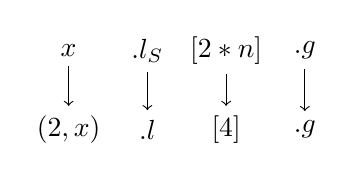
\begin{tikzpicture}
    \node              (a1) {$x$};
    \node[right of=a1] (a2) {$.l_S$};
    \node[right of=a2] (a3) {$[2*n]$};
    \node[right of=a3] (a4) {$.g$};

    \node[below of=a1] (b1) {$(2, x)$};
    \node[below of=a2] (b2) {$.l$};
    \node[below of=a3] (b3) {$[4]$};
    \node[below of=a4] (b4) {$.g$};

    \draw[->] (a1) -- (b1);
    \draw[->] (a2) -- (b2);
    \draw[->] (a3) -- (b3);
    \draw[->] (a4) -- (b4);
  \end{tikzpicture}

  \caption{Évaluation des valeurs gauches}
\label{fig:eval-lv}
\end{figure}%}}}

\section{Expressions}
\label{sec:eval-exp}

Évaluer une constante est le cas le plus simple, puisqu'en quelque sorte
celle-ci est déjà évaluée. À chaque constante syntaxique $c$, on peut associer
une valeur sémantique $\widehat{c}$. Par exemple, au chiffre (symbole) $3$, on
associe le nombre (entier) $\widehat{3}$.

\begin{mathpar}
  \semrule{Exp-Cst}
\end{mathpar}

De même, une fonction est déjà évaluée:

\begin{mathpar}
  \semrule{Exp-Fun}
\end{mathpar}

Pour lire le contenu d'un emplacement mémoire (valeur gauche), il faut tout d'abord
l'évaluer en un chemin.

\begin{mathpar}
  \semrule{Exp-Lv}
\end{mathpar}

Pour évaluer une expression constituée d'un opérateur, on évalue une
sous-expression, puis l'autre (l'ordre d'évaluation, est encore imposé: de
gauche à droite). À chaque opérateur $\opbin$, correspond un opérateur
sémantique $\widehat{\opbin}$ qui agit sur les valeurs. Par exemple, l'opérateur
$\widehat{+}$ est l'addition entre entiers machine
(page~\pageref{page:entiers-bits}). Comme précisé dans la
section~\ref{sec:sem-ops}, la division par zéro via $/$, $\%$ ou $\floatop{/}$
provoque l'erreur $\serr{div}$.

\label{rule:exp-binop}
\begin{mathpar}
  \semrule{Exp-UnOp}

  \semrule{Exp-BinOp}
\end{mathpar}

Il est nécessaire de dire un mot sur les opérations $\widehat{+_p}$ et
$\widehat{-_p}$ définissant l'arithmétique des pointeurs. Celles-ci sont
uniquement définies pour les références mémoire à un tableau, c'est-à-dire
celles qui ont la forme $\widehat{\&}~φ[n]$ (par souci de clarté on ne note pas
tous les~$\widehat{\cdot}$ ci-dessous). On a alors:

\begin{align*}
  \widehat{\&}~φ[n]~+_p~i & = \widehat{\&}~φ[n+i] \\
  \widehat{\&}~φ[n]~-_p~i & = \widehat{\&}~φ[n-i] \\
\end{align*}

Cela implique qu'on ne peut pas faire faire d'arithmétique de pointeurs au sein
d'une même structure. Autrement c'est une erreur de manipulation de pointeurs
\label{page:def-arith-ptr-error}\footnote{
Cela est cohérent avec la norme C99:
\enquote{If the pointer operand points to an element of an array object, and the
    array is large enough, […] ; otherwise, the behavior is undefined.
    }~\cite[6.5.6~§8]{AnsiC}}
et l'opérateur $\widehat{\opbin}$ renvoie $\serr{ptr}$.

Si l'indice calculé ($n+i$ ou $n-i$) sort de l'espace alloué, alors l'erreur
sera faite au moment de l'accès: la lentille $T$ renverra $\serr{array}$
(page~\pageref{subsec:lens-array}).

Pour prendre l'adresse d'une variable, il suffit de résoudre celle-ci dans
l'état mémoire courant.

\begin{mathpar}
  \semrule{Exp-AddrOf}
\end{mathpar}

L'affectation se déroule en 3 étapes. D'abord, l'expression est évaluée en une
valeur $v$. Ensuite, la valeur gauche est évaluée en un chemin $φ$. Enfin, un
nouvel état mémoire est construit, où la valeur accessible par $φ$ est remplacée
par $v$. Comme dans le langage C, l'expression d'affectation produit une valeur,
qui est celle qui a été affectée.

\begin{mathpar}
  \semrule{Exp-Set}
\end{mathpar}

\subsection*{Expressions composées}

Les littéraux de structures sont évalués en leurs constructions syntaxiques
respectives. Puisque les contextes d'évaluation sont de la forme $ [ v_1 ; … ; C
; … ; e_n ] $, l'évaluation se fait toujours de gauche à droite.

\begin{mathpar}
  \semrule{Exp-Struct}

  \semrule{Exp-Array}
\end{mathpar}

%\shorthandoff{!}
%\begin{figure}%{{{

  %\centering

  %\begin{tikzpicture}
    %[node distance=2cm]

    %\node (m0) {$m_0$};
    %\node[right of=m0, node distance=3cm] (m1) {$m_1$};
    %\node[below of=m1]                    (m2) {$m_2$};
    %\node at ($(m0)!(m2)!(0,1)$)          (m3) {$m_3$};
    %\node[below of=m3]                    (m4) {$m_4$};

    %\draw [->] (m0) -- node[auto] {$\mathrm{Push}(\vec{a}↦\vec{v})$}    (m1);
    %\draw [->] (m1) -- node[auto] {$i → \iReturn{v_r}$}                 (m2);
    %\draw [->] (m2) -- node[auto] {$\mathrm{Pop}$}                      (m3);
    %\draw [->] (m3) -- node[auto] {$\mathrm{Cleanup}$}                  (m4);

    %\draw [dashed, ->] ($ (m0) + (-5mm, -3mm) $)
                    %-- node[auto, swap] {$f(\vec{e}) → v$}
                       %($ (m4) + (-5mm, 3mm) $);

  %\end{tikzpicture}

  %\caption[Appel d'une fonction]
  %{ Appel d'une fonction.
    %La taille de la pile croît de gauche à droite,
    %et les réductions se font de haut en bas.
  %}
%\label{fig:fcall-details}

%\end{figure}%}}}
%\shorthandon{!}

L'appel de fonction est traité de la manière suivante. On ne peut pas facilement
relier un pas d'évaluation de $i$ à un pas d'évaluation de $\eFun{a}{i}
(v_1,…,v_n)$, et donc un contexte $C \gramisa \eFun{a}{\ctxEmpty} (v_1,…,v_n)$
n'est pas à considérer. En effet, l'empilement suivi du dépilement modifie la
mémoire.

On emploie donc une règle \textsc{Exp-Call-Ctx} qui relie un pas interne
$\mm{m_1}{i}{m_2}{i'}$ à un pas externe. Une fois l'instruction interne réduite
d'un pas, on évalue les arguments en des valeurs $v'_i$. Ils correspondent aux
nouvelles valeurs à passer à la fonction.

Les autres fonctions permettent de transférer le flot de contrôle: en retournant
la même instruction pour une instruction terminale, ou en propageant une erreur.
Dans le cas où on retourne de la fonction par $i = \iReturn{v}$, il faut alors
supprimer les références aux variables qui ont disparu grâce aux opérateurs
$\phx\cCleanup$ et $\phxx\cV$.

\label{page:return-fonction}
On suppose deux choses sur chaque fonction: d'une part, les noms de ses
arguments sont deux à deux différents et, d'autre part, son corps se termine par
une instruction $\iReturn{\cdot}$. Cela veut dire que la dernière instruction
doit être soit de cette forme, soit par exemple une alternative dans laquelle
les deux branches se terminent par un $\iReturn{\cdot}$. C'est une propriété qui
peut être détectée statiquement avant l'exécution. Néanmoins, dans la syntaxe
concrète, on peut supposer qu'un $\iReturn{\eUnit}$ est inséré automatiquement
en fin de fonction lorsqu'aucun $\iReturn{\cdot}$ n'est présent dans son corps.

\begin{mathpar}
    \semrule{Exp-Call-Ctx}

    \semrule{Exp-Call-Err}

    \semrule{Exp-Call-Return}
\end{mathpar}

\section{Instructions}
\label{sec:eval-instr}

Les cas de la séquence et de l'évaluation d'une expression sont sans surprise.

\begin{mathpar}
  \semrule{Seq}

  \semrule{Exp}
\end{mathpar}

L'évaluation de $\iDecl{x}{v}{i}$ sous $m$ se fait de la manière suivante,
similaire à l'appel de fonction.
La règle principale est \textsc{Decl-Ctx} qui relie un pas d'évaluation sous une
déclaration à un pas d'évaluation externe : pour ce faire, on étend l'état
mémoire en ajoutant $x$, on effectue le pas, puis on enlève $x$. L'instruction
résultante est la déclaration de $x$ avec la nouvelle valeur $v'$ de $x$ après
le pas d'exécution\footnote{
    On peut remarquer qu'il est impossible de définir un contexte d'évaluation
    $C \gramisa \iDecl{x}{v}{C}$. En effet, puisque celui-ci nécessiterait
    d'ajouter une variable, il ne préserve pas la mémoire.
}.

\label{page:decl-masquage}
On suppose qu'il n'y a pas de masquage au sein d'une fonction, c'est-à-dire que
le nom d'une variable déclarée n'est pas visible avant cette déclaration.

Si $i$ est terminale ($\iPass$ ou $\iReturn{v}$), alors on peut s'évaluer en $i$
en nettoyant l'espace mémoire des références à $x$ qui peuvent subsister.

Enfin, si une erreur se produit elle est propagée.

\begin{mathpar}
 \semrule{Decl-Pass}

 \semrule{Decl-Return}

 \semrule{Decl-Ctx}

 \semrule{Decl-Err}
\end{mathpar}

Pour traiter l'alternative, on a besoin de 2 règles. Elles commencent de la même
manière, en évaluant la condition. Si le résultat est 0 (et seulement dans ce
cas), c'est la règle \textsc{If-False} qui est appliquée et l'instruction
revient à évaluer la branche \enquote{\emph{else}}. Dans les autres cas, c'est
la règle \textsc{If-True} qui s'applique et la branche \enquote{\emph{then}} qui
est prise.

\begin{mathpar}
  \semrule{If-False}

  \semrule{If-True}
\end{mathpar}

On exprime la sémantique de la boucle comme une simple règle de réécriture:

\begin{mathpar}
  \semrule{While}
\end{mathpar}

Enfin, si un $\phx\iReturn$ apparaît dans une séquence, on peut supprimer la suite:

\begin{mathpar}
  \semrule{Return}
\end{mathpar}

\section{Erreurs}
\label{sec:eval-errors}

Les erreurs se propagent des données vers l'interprète; c'est-à-dire que si
une expression ou instruction est réduite en une valeur d'erreur $Ω$, alors une
transition est faite vers cet état d'erreur.

Cela est aussi vrai d'une sous-expression ou sous-instruction: si l'évaluation
de $e_1$ provoque une erreur, l'évaluation de $e_1 + e_2$ également. La notion
de sous-expression ou sous instruction est définie en fonction des contextes
$C$. Notons que, dans \textsc{Eval-Err}, $\ctxSub{C}{e}$ peut être une expression
ou une instruction.

\begin{mathpar}
  \semrule{Exp-Err}

  \semrule{Eval-Err}
\end{mathpar}

\section{Phrases et exécution d'un programme}

Un programme est constitué d'une suite de phrases: déclarations de fonctions,
de variables et de types, et évaluation d'expressions.

Donc l'évaluation d'une phrase $p$ fait passer d'un état mémoire $m$
à un autre $m'$, ce que l'on note $\ph{m}{p}{m'}$.

L'évaluation d'une expression est uniquement faite pour ses effets de bord. Par
exemple, après avoir défini les fonctions du programme, on pourra appeler
\texttt{main()}. La déclaration d'une variable globale (avec un initialiseur),
quant à elle, consiste à évaluer cet initialiseur et à étendre l'état mémoire
avec ce couple (variable, valeur). On suppose que les variables globales ont
toutes des noms différents. Notons que ces évaluations se font à grands pas.

Enfin, l'exécution d'un programme est sans surprise l'exécution de ses phrases,
les unes à la suite des autres.

\begin{mathpar}
  \semrule{ET-Exp}

  \semrule{ET-Var}

  \semrule{T*-Nil}

  \semrule{T*-Cons}

  \semrule{Prog}
\end{mathpar}

\section*{Conclusion}

On vient de définir un langage impératif, \langname. Le but est que celui-ci
serve de support à des analyses statiques, afin notamment de montrer une
propriété de sécurité sur les pointeurs. Pour le moment, on a seulement défini
ce que sont les programmes (leur syntaxe) et comment ils s'exécutent (leur
sémantique). Sur ces deux points, on note que nous sommes restés suffisamment
proches de C, tout en utilisant pour la mémoire un modèle plus structuré qu'une
simple suite d'octets. Les définitions de la syntaxe ainsi que de la sémantique
sont rappelées dans l'annexe~\ref{anx:eval} (sections~\ref{sec:anx-sem-start}
à~\ref{sec:anx-sem-end}).

Afin de manipuler les états mémoire dans la sémantique d'évaluation, nous avons
utilisé le concept des lentilles, qui permettent de chaîner des accesseurs entre
eux et d'accéder simplement à des valeurs profondes de la mémoire, en utilisant
le même outil pour la lecture et l'écriture.

Pour le moment, on ne peut rien présager de l'exécution d'un programme bien
formé syntaxiquement. Pour la grande majorité des programmes bien formés (à la
syntaxe correcte), l'évaluation s'arrêtera soit par une erreur, soit parce
qu'aucune règle d'évaluation ne peut s'appliquer. Dans les
chapitres~\ref{cha:typbase} et~\ref{cha:qualifs}, nous allons donc définir un
système de types qui permet de rejeter ces programmes se comportant mal à
l'exécution.

% vim: spelllang=fr
